\documentclass[11pt]{article}
\usepackage[square]{natbib} 
\usepackage{aas_macros}
\usepackage{amsfonts}
\usepackage{amsbsy}
\usepackage{graphicx}

%\documentclass[12pt,preprint]{aastex}
%\documentclass[apj,onecolumn]{emulateapj}
%\usepackage{apjfonts}
%\citestyle{aa}

\usepackage[pdftex,bookmarks=true]{hyperref}

\newcommand{\ang}{\textrm{\scriptsize \AA}}
\newcommand{\photoz}{\textrm{phot-}\textit{z}}
\newcommand{\photozs}{\textrm{phot-}\textit{z}\textrm{s}}
\newcommand{\zphot}{z_\mathrm{phot}}
\newcommand{\zspec}{z_\mathrm{spec}}
\newcommand{\SFR}{\textit{SFR}}
\newcommand{\eazy}{\textsc{EAZY}}
\newcommand{\textterm}[1]{\hspace*{1cm}\textbf{\texttt{\$ #1}}}

%\textheight=23cm
%\textwidth=17.5cm
%\voffset=2cm
%\hoffset=2.5cm
%\vskip 10pt plus 10pt minus 1pt

\textwidth=6.5in
\hoffset=-0.7in
\textheight=9in
\voffset=-1in
\setlength{\parindent}{0cm}
\setlength{\parskip}{0.1cm}
%\setlength{\lineskip}{2cm}

\begin{document}
%\title{\eazy: A Fast, Public Photometric Redshift Code}
%\author{Gabriel Brammer, Pieter van Dokkum, Paolo Coppi}

%\thispagestyle{empty}
\begin{center}
\vfill
%\huge{\eazy:}\Large{\ A Fast, Public Photometric Redshift Code}\\
\huge{\textbf{E}$_\mathrm{asy\ and}$ \textbf{A}$_\mathrm{ccurate}$ \textbf{Z}$_\mathrm{(photometric\ redshifts)\ from}$\textbf{\ Y}$_\mathrm{ale}$ }\\
\ \\
\Large{Gabriel Brammer, Pieter van Dokkum, Paolo Coppi}\\
\small{{Department of Astronomy, Yale University}} \\
\large{\emph{(Incomplete) Draft Version: \today}}\\
\end{center}

%\newpage

\tableofcontents

\newpage

\section{Introduction}

\eazy\ is a public photometric redshift (\photoz) code designed to incorporate
the most recent \photoz\ innovations into a flexible yet easy-to-use interface
(\`a la HyperZ - \cite{hyperz}) with default settings that will produce
high-quality results without significant optimization by the user.  The default
settings have been optimized to work with multi-wavelength photometric data
alone and therefore \eazy\ does not require a large ``calibration set'' of
sources with measured spectroscopic redshifts to obtain optimal \photozs. 
Important features of the code are summarized below:

\begin{itemize}

\item Fitting is done in linear units to naturally handle negative fluxes

\item Fit one, two, or many combinations of templates simultaneously

\item Incorporation of a redshift prior, determined from the ``Millenium
lightcones''

\item Template set optimized on the lightcone photometry

\item Template error function

\item Redshift quality parameter, ``$Q_z$''

\end{itemize}

In the text below, parameters that \eazy\ uses are printed in \textsc{small
caps}, contents of ASCII files are printed in \texttt{typewriter} font, UNIX
terminal commands are shown as, e.g., \textbf{\texttt{\$ ls}},  and literal
filenames are printed in \textit{italics}.  
\ \\
\ \\
This document is intended as a practical guide to setting up and using the \eazy\ software package.  For a higher level discussion of the algorithms summarized below and for extensive tests of the code on publicly-available photometric datasets, see \cite{eazy_paper}.

%\section{Algorithm \label{algorithm}}
%
%The heart of the \eazy\ \photoz\ computation is the standard template-fitting
%algorithm that seeks to minimize 
%
%\begin{equation}
%\chi^2(z) = \sum_{i=1}^{N_\mathrm{filt}} \frac{(F_i - T_i(z))^2}{(\Delta F_i)^2}, \label{chi2}
%\end{equation}
%
%where $N_\mathrm{filt}$ is the number of filters used; $F_i$ is the observed
%flux through filter, $i$; $T_i(z)$ is the ``observed'' model flux integrated
%through filter, $i$, at redshift, $z$; and $\Delta F_i$ is the uncertainty in
%the observed flux (\S\ref{temp_err}).  \eazy\ allows that $T_i$ can be
%calculated for a single template or for non-negative linear combinations of
%multiple templates.  More explicitly,
%
%\begin{equation}
%T_i(z) = \sum_{j=1}^{1 || 2 || \mathrm{all}} \alpha_j \cdot t_{i,j}(z), \label{lincomb1}
%\end{equation}
%
%where the normalization coefficients, $\alpha_j$, are determined for one, two,
%or all of the templates, $t_j$, in the user-supplied list.  For the one- or
%two-template fits, the normalizations are determined analytically using
%least-squares.  \eazy\ does not keep track of the 2-D template/redshift matrix,
%so $T_i(z)$ will represent the best single or pair fit at redshift, $z$. 
%Two-template fits where one of the coefficients $\alpha_j < 0$ are ignored and
%$T_i(z)$ defaults to the best single-template fit if no valid pairs are found
%at redshift, $z$.  In ``all'' mode, the non-negative coefficients for
%$N_\mathrm{temp}$ templates are computed iteratively following the algorithm of
%\cite{nmf}.  See Appendix \ref{details} for details concerning how the template
%SEDs are integrated through the user-supplied filter curves.
%
%    \subsection{Priors \label{priors}}
%
%    \eazy\ incorporates a Bayesian redshift prior \citep{bpz} equal to the
%    redshift distribution of galaxies in lightcones \citep{momaf} computed from
%    semi-analytic models \citep{lightcones}.  The prior probability, $P(z|m_0)$,
%    is computed for a range of apparent magnitude bins and is provided for
%    sources selected in either the $R$ or $K$ band (see Figure 4 of \cite{eazy_paper}).  The prior
%    is multiplied to the redshift probability, $p(z) = \exp
%    \left(-\chi^2/2\right)$,
%
%    \begin{equation}
%    p'(z) = p(z)\cdot P(z|m_0)\ \ . \label{prior_eq1}
%    \end{equation}
%    
%    One can then choose the ``best'' redshift in a number of ways, for example
%    the mode (maximum) of $p'(z)$ or the expectation value
%
%    \begin{equation}
%    \left<z\right> = \frac{\int z\cdot p'(z)\ dz}{\int p'(z)\ dz}\ \ . \label{zm2}
%    \end{equation}
%    
%    \eazy\ outputs both of these options (\S XXX).  Comparing the two values to
%    measured $\zspec$ for sources from a number of $K$-selected catalogs
%    indicates that the scatter in $\zphot-\zspec$ is usually lower for $\zphot
%    = \left<z\right>$ (Eq. \ref{zm2}).
%
%    \subsection{Custom template set \label{font_nmf}}
%    
%    The default template set is based on Pegase \citep{pegase} population synthesis models fit to the synthetic lightcone photometry.  The default behavior for these six templates is to fit them all simultaneously using \textsc{template\_combos=}\textsl{a}.  See \cite{eazy_paper} for more details on how this template set is constructed.  Any user-defined template set can be incorporated by creating a separate \textit{spectra.param} file (\S\ref{s:template_params}).
%    
%    \subsection{Template error function \label{temp_err}}
%    
%    Same here.
    
\section{Installation \label{installation}}
    
\eazy\ does not require a particular directory structure or any environment
variables to be set.  The example below shows the structure of the program
files as they're distributed, but you can put things anywhere you want making
sure to change the appropriate file paths in \textit{zphot.param}.  To get
started, download the tarfile of the distribution from the website,
\begin{center}\url{http://www.astro.yale.edu/eazy/}\end{center}and
unpack it:

\textterm{tar xzvf eazy-1.0.tar.gz       }

Now compile the code and run it:

\textterm{cd eazy-1.0/src}\\
\textterm{make}\\
\textterm{cd ../inputs}\\
\textterm{../src/eazy}
        
And you're done.  Well, not quite yet.  \eazy\ requires a file,
\textit{zphot.param}, in the working directory that contains a list of
parameters for the run.  In this case \eazy\ didn't find the file, so it
created a file for you, \textit{zphot.param.default}, containing all of the
default parameters. We'll use the defaults for this first run on the example
catalog, so do

\textterm{cp zphot.param.default zphot.param}\\
\textterm{../src/eazy}
 
Now you're done and you have computed \photozs\ for the HDF-N catalog of
\cite{hdfn} with $\sigma_z/(1+\zspec) \sim 0.04$.  \eazy\ dumps a lot of
information to the terminal so you can see what it's up to.  For some UNIX
terminals, printing to the screen can take up a significant fraction of the CPU
time, so you might want to pipe the output to a file (where you can then
actually read it):

\textterm{../src/eazy > logfile}

\section{Parameters and input files \label{params}}

\subsection{\textit{zphot.param} \label{zphot.param}} This is the main ASCII file
that contains the parameters needed to run \eazy\.  The code is not too picky
about the formatting of this file; it just looks for lines formatted like \\
\hspace*{1cm}\textsc{parameter}\ \ \ \ \ \textit{\texttt{value}}\ \ [\# \textsc{optional comment}]\\ and assigns
the value to the parameter if the parameter is one that \eazy\ recognizes.  If the
parameter is not recognized, the line is ignored.  If a parameter from the full
list shown in the ``default'' file is not found in the user-supplied
\textit{zphot.param} file, then the default value is used.  All of the parameters
that \eazy\ recognizes and their default values are described below.

\subsubsection{Filters}
%\begin{itemize}
\begin{tabular}{ll}
 \textsc{FILTERS\_RES} & \textsl{  master.FILTERS.RES} \\
 \textsc{FILTER\_FORMAT} & \textsl{         1} \\
 \textsc{SMOOTH\_FILTERS} & \textsl{        yes} \\
 \textsc{SMOOTH\_SIGMA} & \textsl{        100.}
\end{tabular}

\vspace*{0.5cm}\textsc{filters\_res} is a text file containing filter response
curves, formatted in the same way as the \textsc{HyperZ} filter response file. 
\eazy\ is not able to combine multiple entries (e.g. filter$\times$detector)
from the response file.  Each filter entry consists of a header line showing a)
the number of subsequent lines, $N_R$, that define the filter response and b) a
short description of the filter.  The header line is followed by $N_R$ lines of
three columns: $i,\ \lambda_i/$\AA$,\ R_i(\lambda)$:

\begin{verbatim}
    ...
  503 41580.0 0.000146
  504 41620.0 0.000116
  505 41650.0 0.000182
427     IRAC_c2 BAND2 total system response (SIRTF/IRAC Web site) 4.5micron (ch2)
  1 37040.0 0.000458
  2 37070.0 0.000398
  3 37090.0 0.000344
    ...
\end{verbatim}

\noindent See \S\ref{s:input_files} and \S\ref{s:translate} for how to tell
\eazy\ which of the filters in the \textsc{filters\_res} file correspond to
which column in your photometric catalog file.

\textsc{filter\_format} tells the program if the response curves provided in
the \textsc{filters\_res} file are determined for energy-counting
(\textsc{filter\_format}=0) or photon-counting (\textsc{filter\_format}=1)
detectors.  Most modern response curves (via e.g. the ESO ETC webpages or 
\textsc{synphot}) are for photon-counting detectors (CCDs), while some older
response curves available in the literature may be in the other format (without
necessarily saying so; see also Appendix \ref{details} or the appendix of
\cite{maiz} for more information).\\

If \textsc{smooth\_filters} is set, then the response curve $R(\lambda)$ is
smoothed with a gaussian with width $\sigma =\ $\textsc{smooth\_sigma}$\cdot$1\
\AA:
\begin{equation}
\Re_i = \frac{1}{b_i}\sum_{j=1}^{N_R} R_i \cdot \exp\left[\frac{\left(\lambda_i-\lambda_j\right)^2}{2\sigma^2}\right] \label{smooth_filters},
\end{equation}
where $b_i = \sum_{j=1}^{N_R} \exp[(\lambda_i-\lambda_j)^2/2\sigma^2]$.

%\end{itemize}

\subsubsection{Templates} \label{s:template_params}
\begin{tabular}{ll}
 \textsc{TEMPLATES\_FILE} & \textsl{       ../templates/font\_nmf.spectra.param } \\
 \textsc{TEMPLATE\_COMBOS } & \textsl{     a                } \\
 \textsc{NMF\_TOLERANCE} & \textsl{        1.e-4           } \\
\end{tabular}
\vspace*{0.5cm}

\textsc{templates\_file} is a text file containing a list of the template
filenames you wish to use to compute photometric redshifts.  The default file
is shown below.  \textsc{template\_combos} specifies the number of templates to
combine with non-negative coefficients, $\alpha_i$, as in Eq. 2 of \cite{eazy_paper}.  

\vspace*{0.25cm}
\begin{tabular}{lrl}
 \textsc{template\_combos}\ =&1 &  \textrm{single template fit} \\
 &2 & \textrm{pairs of templates as defined in \textsc{templates\_file}}\\
 & $-2$ & \textrm{all pair combinations} \\
 &$(a\ \mathrm{or}\ 99)$ &  \textrm{all templates in \textsc{templates\_file} simultaneously}
\end{tabular}

\vspace*{0.25cm} For fits with single or pairs of templates, $\alpha_i$ are
computed analytically following e.g. \cite{bevington} (Appendix
\ref{app_lincomb}).  Fitting all of the templates simultaneously, $\alpha_i$
must be computed iteratively, and the iteration tolerance is controlled by the
\textsc{nmf\_tolerance} parameter.  The default value of this parameter
reflects a compromise between increasing $\chi^2$ for the template fits when
using larger values and increasing computation time for smaller values.

\vspace*{0.25cm}\textsc{(templates\_file)}\vspace*{-0.4cm}
\begin{verbatim}
    1   ../templates/font_nmf/font_5_t1.dat    1.0 0 1.0   2,3,4,5
    2   ../templates/font_nmf/font_5_t2.dat    1.0 0 1.0   3,4,5
    3   ../templates/font_nmf/font_5_t3.dat    1.0 0 1.0   4,5
    4   ../templates/font_nmf/font_5_t4.dat    1.0 0 1.0   5
    5   ../templates/font_nmf/font_5_t5.dat    1.0 0 1.0   
\end{verbatim}

The first column is a running count of the files in the template list and is
used to identify the templates in the output files.  The second column is the
relative path from the working directory to the individual template file, which
is an ASCII file containing two columns: \textbf{1) $\lambda$ and 2) flux in
$F_\lambda$} (arbitrarily normalized).  The third column is multiplied to the
template wavelengths to scale them to \AA;  for example, if $\lambda$ in the
template file is specified in $\mu$m, this column should be $1.e4$.  The fourth
column is the ``age'' of the template, in Gyr.  If this column is set to
something other than zero, then the code will only use this template at
redshifts where the age of the universe is greater than the age of the
template.  The fifth column is currently not used by the code.  The final column is
a comma-separated list of the ID numbers of the other templates that will be
combined with the current template if \textsc{template\_combos}=2.

\vspace*{0.5cm}
\begin{tabular}{ll} 
 \textsc{WAVELENGTH\_FILE } & \textsl{     lambda.def       } \\
 \textsc{TEMP\_ERR\_FILE} & \textsl{       best\_temp\_err\_v1.out } \\
 \textsc{TEMP\_ERR\_A2 } & \textsl{         1.00              } \\
 \textsc{SYS\_ERR    } & \textsl{          0.00               } \\
 \textsc{APPLY\_IGM   } & \textsl{         y                  } \\
\end{tabular}

\vspace*{0.25cm}All of the templates are rebinned to the (rest-frame)
wavelength grid defined in the \textsc{wavelength\_file} (Appendix
\ref{details}).  The supplied file, \textit{lambda.def}, is a roughly
logarithmic grid from 100 \AA to 11 $\mu$m to allow fits to \textit{rest-frame}
NUV and NIR photometry at high- and low-$z$, respectively.  \eazy\ will ignore
redshifts where filters fall off of the template or \textsc{wavelength\_file}
grids in the observed frame.

\textsc{temp\_err\_file} is an ASCII file containing the rest-frame template
error function described in \cite{eazy_paper}.  \eazy\ reads the first two
columns of this file, $\lambda_\mathrm{te}$ and $\sigma_\mathrm{te}(\lambda)$. 
\textsc{temp\_err\_a2} is multiplied to $\sigma_\mathrm{te}$, so you can easily
turn off the effects of the template error function by setting
\textsc{temp\_err\_a2}=0.  \textsc{sys\_err} can be used as a minimum
fractional error error that is added to the uncertainties equally for every
filter and at every redshift.  The total flux uncertainty in filter, $j$, in
Eq. 1 of \cite{eazy_paper} is 

\begin{equation}
(\delta F_j)^2 = \sigma_{j,\mathrm{cat}}^2 + F_j^2 \left[\sigma_\mathrm{sys}^2+\left(\textsc{temp\_err\_a2}\cdot\sigma_\mathrm{te}(\lambda_{j})\right)^2\right], \label{full_error}
\end{equation}

where $\sigma_{i,\mathrm{cat}}$ is the flux uncertainty from the photometric
catalog and $\sigma_\mathrm{te}(\lambda_{i})$ is the template error
interpolated at the rest-frame central wavelength of filter, $i$.

If \textsc{apply\_igm} is set, then IGM absorption in the FUV is applied to the
templates following \cite{madau95}.

\vspace*{0.25cm}\begin{tabular}{ll}
 \textsc{DUMP\_TEMPLATE\_CACHE} & \textsl{  n                 } \\
 \textsc{USE\_TEMPLATE\_CACHE  } & \textsl{ n                 } \\
 \textsc{CACHE\_FILE       } & \textsl{    tempfilt.dat       } 
\end{tabular}

\vspace*{0.25cm}You can dump the 3D [template][filter][redshift] matrix to a
file, \textsc{cache\_file}, to avoid computing it every time you run the code. 
This is most useful when using lists of hundreds of templates, but be careful
when using the template cache files because \eazy\ is not smart enough to know
if the parameters that were used to generate the cache were the same as the
parameters of the current run.

\subsubsection{Input Files} \label{s:input_files}
\begin{tabular}{ll}
 \textsc{CATALOG\_FILE     } & \textsl{    hdfn\_fs99\_eazy.cat      } \\
 \textsc{NOT\_OBS\_THRESHOLD } & \textsl{   -90                } \\
 \textsc{N\_MIN\_COLORS      } & \textsl{   5                 } 
\end{tabular}

\vspace*{0.25cm}\textsc{catalog\_file} is the input photometric catalog that
contains photometric fluxes and uncertainties observed in $N_\mathrm{filt}$
filters.  The first line of this file must contain the column names for as many
columns as you want the program to read.  The column names can be any string,
but \eazy\ will only recognize columns with (case-sensitive) names
\{\textsl{id,z\_spec,Fn,En,TOTn}\}---see also \textit{zphot.translate},
\S\ref{s:translate}.  Column, \textsl{id}, is just used to identify objects in
the output files.  Column, \textsl{z\_spec}, is used when setting
\textsc{fix\_zspec} and the values in this column are printed in the
\textit{zout} output file.  The columns, \textsl{Fn} and \textsl{En}, are the
$\mathbf{F_\nu}$ flux and error columns for filter \textsl{n}, respectively. 
Again, by convention \textbf{the photometric fluxes and errors are given in
units of $F_\nu$ while the template SEDs are provided in $F_\lambda$}.  The
number \textsl{n} following \textsl{F} or \textsl{E} refers to the order of the
filters in the \textsc{filters\_res} file.  For example, in the HDF-N catalog
provided with the \eazy\ distribution, the second column is the WFPC2
\textsl{F300W} flux and the \textsl{F300W} filter curve is the 10th entry in
the \textsc{filters\_res} file, so the name for this column in the header line
should be \textsl{F10}.  If ``color'' and ``total'' fluxes are provided in the
photometric catalog (e.g. FIRES), the \textsl{TOTn} column can be used to
compute the color$\rightarrow$total scaling and \textsl{n} for the TOT column
must match one of the \textsl{Fn/En} pairs.

If an object has missing data for some reason in a particular filter, the flux
value should be set to some large negative number in the photometric
catalog---a number that is more negative than \textsc{not\_obs\_threshold}. 
This value should be more negative than any \textit{measured} negative flux is
expected to be, since \eazy\ naturally handles non-detections with negative
fluxes.  \eazy\ will skip any object in the catalog with fewer than
\textsc{n\_min\_colors} filters with \textsl{Fn}$\ >\
$\textsc{not\_obs\_threshold}.

\subsubsection{Output Files}
\begin{tabular}{ll}
 \textsc{OUTPUT\_DIRECTORY  } & \textsl{   OUTPUT             } \\
 \textsc{MAIN\_OUTPUT\_FILE   } & \textsl{  photz             } \\
 \textsc{PRINT\_ERRORS   } & \textsl{      y                  } \\
 \textsc{VERBOSE\_LOG   } & \textsl{       y                  } \\
 \textsc{OBS\_SED\_FILE   } & \textsl{      n                 } \\
 \textsc{TEMP\_SED\_FILE   } & \textsl{     n                 } \\
 \textsc{POFZ\_FILE        } & \textsl{    n                  } \\
 \textsc{BINARY\_OUTPUT        } & \textsl{    n                  } 
\end{tabular}

See \S\ref{all_output} for descriptions of the contents of the output files,
which are all placed in the \textsc{output\_directory}.  

\subsubsection{Redshift+Magnitude prior}
\begin{tabular}{ll}
 \textsc{APPLY\_PRIOR     } & \textsl{     y                  } \\
 \textsc{PRIOR\_FILE       } & \textsl{    prior\_K\_zmax7.dat  } \\
 \textsc{PRIOR\_FILTER     } & \textsl{    28                 } \\
 \textsc{PRIOR\_ABZP      } & \textsl{     25.0               } 
\end{tabular}

\vspace*{0.25cm}Set \textsc{apply\_prior}=\textsl{y} to use the
redshift/magnitude prior described in \cite{eazy_paper}.  The priors are defined
in the \textsc{prior\_file}, which has one column for $z$ and additional
columns $P(z|m)$ for each (AB) apparent magnitude bin as defined in the first
line of the file.  The apparent magnitude in filter \textsl{n}\ =
\textsc{prior\_filter} is computed for each object from the catalog flux using
\begin{equation}
m_\mathrm{AB} = \textsc{prior\_abzp} - 2.5\log_{10} F_n\ 
\label{prior_mag}
\end{equation}
(For catalog fluxes in $\mu$Jy, \textsc{prior\_abzp}=23.9), and the appropriate
$P(z|m_\mathrm{AB})$ is chosen and applied as in Eq. 4 of \cite{eazy_paper}.

\subsubsection{Redshift Grid}
\begin{tabular}{ll}
 \textsc{FIX\_ZSPEC     } & \textsl{       n                  } \\
 \textsc{Z\_MIN         } & \textsl{       0.01               } \\
 \textsc{Z\_MAX         } & \textsl{       4.0                } \\
 \textsc{Z\_STEP        } & \textsl{       0.01               } \\
 \textsc{Z\_STEP\_TYPE  } & \textsl{        1                 }
\end{tabular}

\vspace*{0.25cm}The templates will be fit according to Eqs. 1 and
2 of \cite{eazy_paper} at redshift values in a grid defined by the parameters above. 
The grid step size will be set following

\vspace*{0.25cm}\begin{tabular}{lcl}
\textsc{z\_step\_type}\ = & 0; & step = \textsc{z\_step} \\
 & 1; & step = \textsc{z\_step}$\times(1+z)$
\end{tabular}

\vspace*{0.25cm}If \textsc{fix\_zspec}=\textsl{y} then \eazy\ looks for a
column, \textsl{z\_spec}, in the \textsc{catalog\_file}.  The template set will
then be fit following \textsc{template\_combos} to the photometry of each
object at the redshift in the redshift grid nearest to \textsl{z\_spec}.


\subsubsection{Zeropoint Offsets}
\begin{tabular}{ll}
 \textsc{GET\_ZP\_OFFSETS   } & \textsl{    n                 } \\
 \textsc{ZP\_OFFSET\_TOL    } & \textsl{    1.e-4             } 
\end{tabular}

\vspace*{0.25cm} If \textsc{get\_zp\_offsets}=\textsl{y} then \eazy\ will look
for a file, \textit{zphot.zeropoint}, and apply zeropoint offsets to the
catalog photometry (\S\ref{zeropoint}).

\subsubsection{Cosmology}
\begin{tabular}{ll}
 \textsc{H0               } & \textsl{    70.0               } \\
 \textsc{OMEGA\_M         } & \textsl{     0.3               } \\
 \textsc{OMEGA\_L       } & \textsl{        0.7               }
\end{tabular}

\vspace*{0.25cm} These parameters are used to compute the age of the universe
at redshift, $z$, to compare with the template ages (optionally) specified in
the \textsc{templates\_file}.  \textsc{H0} is in units of km/s/Mpc and the
\textsc{omega} parameters are the matter and dark energy densities in units of
the critical density.

    \subsection{\textit{zphot.translate} \label{s:translate}}

	This file ``translates'' the column names in
	\textsc{catalog\_file} to the required F\textsl{n} and
	E\textsl{n} formats needed to tell \eazy\ which filter
	corresponds to which columns in the catalog
	(\S\ref{s:input_files}).  Using this file allows you to
	avoid having to edit large catalog files and allows the
	column names in the catalog to be more meaningful and
	not tied to a specific \textsc{filters\_res} file.  The
	format of this file is simply two columns, the first
	being the column name in the \textsc{catalog\_file} and
	the second containing what you want to ``translate'' it
	to (case sensitive).  For example, imagine you have a
	(rather useless) catalog that looks like the following:

\texttt{\# id   zsp    f\_f300w   e\_f300w }\\
\texttt{\   1   1.9     1.00       0.100 }

We need to tell \eazy\ that the 3rd and 4th columns
correspond to fluxes and errors measured in the WFPC2 F300W
filter (number 10 in our \textsc{filters\_res} file).  You
could either edit the catalog to look like:

\texttt{\# id   zsp      F10        E10 }\\
\texttt{\   1   1.9     1.00       0.100 }

or make a \textit{zphot.translate} file like this:

\noindent \texttt{ f\_f300w   F10}\\
\texttt{ e\_f300w  E10}

Note that the spectroscopic redshift column isn't required,
but if you want \eazy\ to recognize it it has to be called
\texttt{z\_spec}.  So you could add an additional line to
the \textit{zphot.translate} file:

\texttt{  zsp  z\_spec}.

    \subsection{\textit{zphot.zeropoint} \label{zeropoint}}
    
	While iterative adjustment of photometric zeropoints is
	not supported in the current version of \eazy\, you can
	specify a separate file that will apply zeropoint
	offsets to the flux and error columns in the the
	\textsc{catalog\_file}.  For example, if you want to
	multiply the flux and error of filter $j$ by a factor of
	1.03 or apply a magnitude offset of +0.07 mag to filter
	$k$, you could make a \textit{zphot.zeropoint} file like
	the following:

\texttt{F\textit{j}\ \ \ 1.03\\M\textit{k}\ \ \ 0.07}

noting the ``F'' and ``M'' as needed for flux or mag offsets and
where $j, k$ are the appropriate filter ID numbers from the
\textsc{filters\_res} file.


\section{Output files \label{all_output}}
  
    \subsection{\textrm{OUTPUT\_FILE.}\textit{zout} \label{zout}}
    
	This is the main output file where the photometric
	redshift information is placed.  The number of columns
	in this file depends somewhat on the number of template
	linear combinations used (\textsc{template\_combos}).

\begin{itemize}

\item \texttt{id}: ID column taken from the input catalog, if it exists

\item \texttt{z\_spec}:  Column of spectroscopic redshifts
taken from input catalog, if it exists.  This is useful for
plotting and comparisons to the computed $z_\mathrm{phot}$,
but otherwise not used within \eazy\ (unless
\textsc{fix\_zspec=y}).

\item \texttt{\{z\_1, z\_2, z\_a\}}: Redshift where $\chi^2$
is minimized for the one-, two-, or all-template linear
combination modes, \textit{before applying the prior}.

\item \texttt{z\_m1}: Redshift marginalized over $p(z|C) = \exp\{-0.5 \chi^2\}$, given by 

\begin{equation}
\mathtt{z\_m1} = \int z\cdot p(z|C)\ dz, \label{zm1}
\end{equation}

\noindent  where $\int p(z|C) dz$ is normalized to unity.

\item \texttt{\{chi\_1, chi\_2, chi\_a\}}: (minimum)
$\chi^2$ value at $z=$\texttt{\{z\_1, z\_2, z\_a\}}

\item \texttt{\{temp\_1, temp\_2a/temp\_2b\}}: Best fit
template ID numbers at $z=$\texttt{\{z\_1, z\_2\}} for the
one- or two- template fits.

\item \texttt{z\_p}: Redshift where likelihood is maximized
($\chi^2$ is minimized) \textit{after} applying the prior,
$p(z|m_0)$.

\item \texttt{chi\_p}: \textit{Original} $\chi^2$ at $z=$\texttt{z\_p}.

\item \texttt{\{temp\_p, temp\_pa/temp\_pb\}}: Best fit
template ID numbers at $z=$\texttt{z\_p} for the one- or
two- template fits.

\item \texttt{z\_m2}: Redshift marginalized over $p(z|C,
m_0) =p(z|C) \cdot p(z|m_0)$, given by

\begin{equation}
\mathtt{z\_m2} = \int z\cdot p(z|C,m0)\ dz, \label{zm2}
\end{equation}

\noindent which includes the prior and where $\int p(z|C,m_0)\ dz$ is normalized to unity.\\
\ \\
$\star\star$\\
 \texttt{z\_m2} usually provides the best photoz estimate
 and allows you to use a coarser redshift grid, which speeds
 up the computation significantly.  That is, \texttt{z\_m2}
 computed with \textsc{z\_step=0.03} is usually very similar
 to \texttt{z\_p} computed with \textsc{z\_step=0.005}. 
 Note, however that in practice the integral in Eq.
 \ref{zm2} assumes that $\lim_{z\to{\textsc{zmin}}}
 p(z)=\lim_{z\to{\textsc{zmax}}} p(z)=0$.  If this isn't
 true, \texttt{z\_m2} (and \texttt{z\_m1}) will be biased
 from edge effects.\\
$\star\star$

\item \texttt{odds}:  Redshift quality parameter, $p_{\Delta
z}$ or ``odds'', from \cite{bpz}, that represents the
fraction of the total integrated probability that lies
within $\pm \Delta z$ of the zphot estimate, and is designed
to identify sources that have broad and/or multi-modal
probability distributions.  Here we use $\Delta z=0.2$.

\item \texttt{\{l68, u68, l95, u95, l99, u99\}}: If
\textsc{print\_errors}=\textsl{y} then these columns are printed, representing
the 1,2, and 3$\sigma$ confidence intervals computed from the $p(z)$ probability
distributions \citep[\S2.5, ][]{eazy_paper}.

\item \texttt{nfilt}: Number of filters, $j$, used in the fit, with flux, 
\begin{equation} \mathrm{F}j > \textsc{not\_obs\_threshold}
\end{equation}


\end{itemize}


    \subsection{\textrm{OUTPUT\_FILE.}\textit{param}}

	This file is created if \textsc{verbose\_log=1} and it
	contains all of the parameter values from
	\textit{zphot.param} used to compute
	\textrm{OUTPUT\_FILE.}\textit{zout}, as well as
	information on the individual filters and templates
	used.  This file itself can be used to recompute the
	photozs just by copying it to \textit{zphot.param} in
	your working directory.
    
  \subsection{\textsl{[ID].}\textit{obs\_sed} \label{obs_sed}}
  
  If \textsc{obs\_sed\_file}=\textsl{y} then an ASCII file will be created for each
  object in the catalog containing the catalog and best-fit template fluxes in each filter, with columns
  
  \begin{itemize}
  
    \item \texttt{lambda}: central wavelength of the (normalized) filter transmission,

    \begin{equation} \texttt{lambda} = \int \lambda\cdot R(\lambda)\ d\lambda \end{equation}

    \item \texttt{flux\_cat}: object flux taken directly from the catalog

    \item \texttt{err\_full}: total error used in the fit (Eq.\ref{full_error})

    \item \texttt{temp[1,2,a]\_z}: normalized template fluxes integrated through the filters at $z=$\texttt{z\_[1,2,a]} (best redshift \textit{without} the prior)

    \item \texttt{temp[1,2,a]\_zprior}: normalized template fluxes integrated through the filters at $z=$\texttt{z\_p} (best redshift \textit{with} the prior)
    
  \end{itemize}
  
  \subsection{\textsl{[ID].}\textit{temp\_sed} \label{temp_sed}}

  If \textsc{temp\_sed\_file}=\textsl{y} then an ASCII file will be created for
  each object in the catalog containing the full redshifted template SEDs
  converted to $F_\nu$, normalized to the object fluxes, and including the IGM
  absorption if \textsc{apply\_igm}=\textsl{y}.  You should be able to plot
  these SEDs directly on top of the ($F_\nu$) catalog fluxes.  The columns in
  this file are
    
  \begin{itemize}

    \item \texttt{lambda}: wavelength as defined in \textsc{wavelength\_file} multiplied by $(1+\texttt{z\_[1,2,a]})$ 

    \item \texttt{tempflux}: full best-fit SED at $z=\texttt{z\_[1,2,a]}$.

    \item \texttt{lambda\_zprior}: wavelength as defined in \textsc{wavelength\_file} multiplied by $(1+\texttt{z\_p})$ 

    \item \texttt{tempflux\_zprior}: full best-fit SED at $z=\texttt{z\_p}$
    
  \end{itemize}
  
  \noindent \textit{N.B.}: The best-fit normalization coefficients for each
  template in \textsc{templates\_file} are given in the header of the
  \textit{temp\_sed} file.
  
  \subsection{\textsl{[ID].}\textit{pz} \label{pz}}
    
  If \textsc{pofz\_file}=\textsl{y} then an ASCII file will be created for each
  object in the catalog containing $p(z)$.  The columns of this file are:
    
  \begin{itemize}
    
    \item \texttt{z}: redshift as computed from the grid parameters
    
    \item \texttt{chi2}: $\chi^2$ from the fit at redshift, $z$.

    \item \texttt{prior}: $p(z|m_0)$ extracted from \textsc{prior\_file},
    printed if \textsc{apply\_prior}=\textsl{y}.

    \item \texttt{pz}: $p(z|C, m_0)$, printed if \textsc{apply\_prior}=\textsl{y}.

    \item \texttt{\{t1, t2a/t2b\}}: Best-fit template ID numbers at redshift,
    $z$, printed if \textsc{template\_combos}=\textsl{1} or \textsl{2}.
 
  \end{itemize}

  \subsection{\textsc{BINARY\_OUTPUT}=\textsl{y}} \label{binary_output}
  
  For even modest numbers of catalog objects, writing the \textit{obs\_sed},
  \textit{temp\_sed}, and \textit{pz} files for each object can quickly take up
  large amounts of disk space and the file IO can significantly slow down the
  execution of the code, to say nothing about having thousands of files to deal
  with. All of these problems can be addressed by writing this output
  information into binary files from which all of the same information can be
  extracted as from the ASCII files.  Setting \textsc{binary\_output}=\textsl{y}
  will create a number of binary files in the output directory in lieu of the
  ASCII files described above.  The binary files can be read by IDL for
  plotting, etc.  An IDL program file is created in the output directory,
  $[].readbin.pro$, that demonstrates how to read the binary files.  See the
  auxiliary file, $sed.pro$, for an example on how to overplot best-fit template
  SEDs on top of observed fluxes.
  
  \ \\
  $NB$: For a test catalog of 1000 objects and 6 filters, running \eazy\ with all of
  the ASCII outputs set took 27 s and created 96 Mb in 3000 output files.  In
  contrast, with \textsc{BINARY\_OUTPUT}=\textsl{y}, \eazy\ took 19 s to run and
  created 1.8 Mb in six output files.
  
%\section{[[IDL routines for plotting results]] \label{idl}}
%
%    \subsection{\textit{show\_fit.pro}}
%
%    \subsection{\textit{freadfile.pro}}
%    
%    \subsection{\textit{sed.pro}}

\begin{thebibliography}{}

\bibitem[Ben{\'{\i}}tez(2000)]{bpz} Ben{\'{\i}}tez, N.\ 
2000, \apj, 536, 571 

\bibitem[Bevington \& Robinson(2003)]{bevington} Bevington, 
P.~R., \& Robinson, D.~K.\ 2003, Data reduction and error analysis for the 
physical sciences, 3rd ed., by Philip R.~Bevington, and Keith 
D.~Robinson.~Boston, MA: McGraw-Hill, ISBN 0-07-247227-8, 2003., 

\bibitem[Blaizot et al.(2005)]{momaf} Blaizot, J., Wadadekar, 
Y., Guiderdoni, B., Colombi, S.~T., Bertin, E., Bouchet, F.~R., Devriendt, 
J.~E.~G., \& Hatton, S.\ 2005, \mnras, 360, 159 

\bibitem[Bolzonella et al.(2000)]{hyperz} Bolzonella, M., 
Miralles, J.-M., \& Pell{\'o}, R.\ 2000, \aap, 363, 476 

\bibitem[Brammer, van Dokkum \& Coppi(2008)]{eazy_paper} Brammer, G., van Dokkum, P.~G., \& Coppi, P.\ 2008, \apj, submitted

\bibitem[De Lucia \& Blaizot(2007)]{lightcones} De Lucia, G., \& 
Blaizot, J.\ 2007, \mnras, 375, 2 

\bibitem[Fern{\'a}ndez-Soto et al.(1999)]{hdfn} 
Fern{\'a}ndez-Soto, A., Lanzetta, K.~M., \& Yahil, A.\ 1999, \apj, 513, 34 

\bibitem[Fioc \& Rocca-Volmerange(1997)]{pegase} Fioc, M., \& 
Rocca-Volmerange, B.\ 1997, \aap, 326, 950 

\bibitem[Madau(1995)]{madau95} Madau, P.\ 1995, \apj, 441, 18 

\bibitem[Ma{\'{\i}}z Apell{\'a}niz(2006)]{maiz} Ma{\'{\i}}z 
Apell{\'a}niz, J.\ 2006, \aj, 131, 1184 

\bibitem[Sha et al.(2007)]{nmf}
Sha, F., Lin, Y., Saul, L.~K., \& Lee, D.~D.\ 2007, Neural Computation, 19, 2004

\end{thebibliography}

\appendix

\section{Interpolation and integration \label{details}}

%Write out in detail how the interpolation and integration is done, as in Ivo's
%webpage.

\begin{figure}
\centering
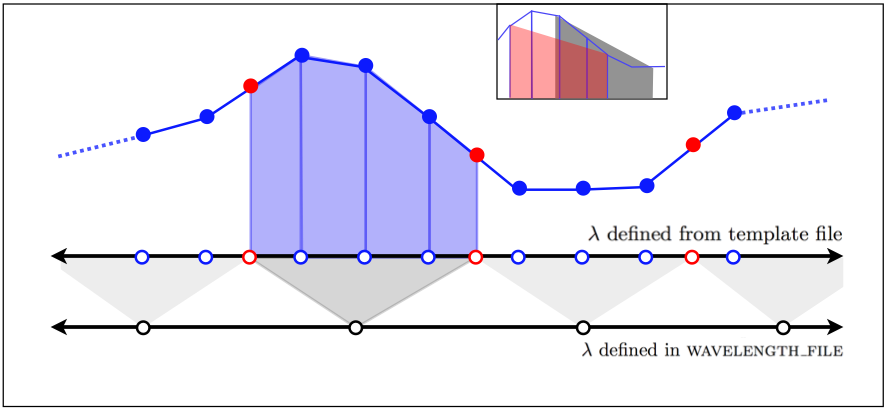
\includegraphics[width=5in]{interp.png}
\caption{Interpolating the input template spectra to the master wavelength grid
defined in the \textsc{wavelength\_file}.}
\label{fig:interp}
\end{figure}

All of the integrations of the filter fluxes, probability distributions, etc.
are done using a simple implementation of the trapezoid rule.  We interpolate
the user-defined template SEDs (with arbitrary wavelength sampling) to a common
(rest-frame) wavelength grid defined in the \textsc{wavelength\_file}, using a
robust interpolation algorithm that preserves flux, shown in Figure
\ref{fig:interp}.  In the figure,  the black circles are the semi-regular
wavelength points defined in the file specified by the \textsc{wavelength\_file}
parameter, and the red points are the midpoints of this wavelength grid.  The
blue points represent the (arbitrary) wavelength grid of a user-supplied
template file, which, in the case of synthetic templates, is generally more
finely sampled than the \textsc{wavelength\_file} grid.  We use the trapezoid
rule (shaded blue regions) to integrate between the linear-interpolated
midpoints and the adjascent template wavelength point, between the intervening
template points, and finally between the last template wavelength point and the
next midpoint.  If there are no template points between the midpoints, we simply
integrate between the midpoints. The inset shows two other simpler integration
schemes that only integrate between the master grid points.  If the curvature is
significant between the master wavelength points, the interpolated flux can
significantly under- or overestimate the true template fluxes.  Systematic
errors in the integrated template fluxes of order a few percent can result in
systematic errors in the derived photometric redshifts.


\section{Linear combinations \label{app_lincomb}}

%Provide details on how the linear combination amplitudes are computed
%analytically for the 1/2 template mode and also explain the \cite{nmf} algorithm
%as it's implemented.

\eazy\ provides the option of fitting (positive) linear combinations of the
templates specified in the \textsc{templates\_file} (\S\ref{s:template_params}) to the
object photometry defined in the catalog.  The normalization coefficients for
either one or two template fits are calculated analytically, while the
normalizations for ``$N$''-template fits are fit iteratively following the
algorithm of \cite{nmf}.

\subsection{Single template fit}

The normalization of each template, $\alpha_i$, at redshift, $z$, is computed
from the sum over \textsc{NFILT} filters, $j$, following
\begin{equation}
\alpha_i = \frac{ \displaystyle\sum_{j}
             \left({T_{z,i,j}\cdot F_j}\right)/\left(\delta F_j\right)^2}
           {\displaystyle\sum_j T_{z,i,j}^2/\left(\delta F_j\right)^2}, \label{eq:alpha1}
\end{equation}

\noindent where $T_{z,i,j}$ is the integrated template flux and $\delta F_j$ is
the full error as defined in Eq. \ref{full_error}.  

\subsection{Two template fit}

The two-template normalizations for templates $i_1$ and $i_2$ are computed analytically using least squares as follows.

\begin{equation}
\mathcal{T} = \left[
\begin {array}{cccc}
T_{z,i_1,0}& T_{z,i_1,1} & \ldots & T_{z,i_1,\textsc{nfilt}} \\
\noalign{\medskip}
T_{z,i_2,0}& T_{z,i_2,1} & \ldots & T_{z,i_2,\textsc{nfilt}} \\
\end {array}
\right]
\;,\ \ \  \mathcal{F} = \left[
\begin {array}{cccc}
F_0 & F_1 & \ldots & F_\textsc{nfilt} \\
\end {array}
\right]
\end{equation}

\begin{equation}
A = \mathcal{T}\mathcal{T}^\mathrm{T},\ \ \ 
\mathbf{b} = \mathcal{T}\cdot\mathcal{F}
\end{equation}

\noindent and 

\begin{equation}
\left(\alpha_{i_1},\ \alpha_{i_2}\right) = A^{-1}\mathbf{b}\ .
\end{equation}

Note that each of the template ($T$) and observed ($F$) fluxes above in filter
$j$ is weighted by $1/\delta F_j^2$. If one of the template amplitudes,
$\alpha_{i_1}$ or $\alpha_{i_2}$, is negative, then the best \textit{single}
template fit is used at redshift, $z$.

\subsection{$N$ template fit}

We use the remarkably simple algorithm of \cite{nmf} to compute the
\textit{non-negative} template normalizations for $\textsc{ntemp}>2$ template
fits.

\begin{equation}
\mathcal{T} = \left[
\begin {array}{cccc}
T_{z,0,0}& T_{z,0,1} & \ldots & T_{z,0,\textsc{nfilt}} \\
\noalign{\medskip}
T_{z,1,0}& T_{z,1,1} & \ldots & T_{z,1,\textsc{nfilt}} \\
\noalign{\medskip}
\vdots & \vdots & \ddots & \vdots \\
\noalign{\medskip}
T_{z,\textsc{ntemp},0}& T_{z,\textsc{ntemp},1} & \ldots & T_{z,\textsc{ntemp},\textsc{nfilt}} \\
\end {array}
\right]
\;,\ \ \  \mathcal{F} = \left[
\begin {array}{cccc}
F_0 & F_1 & \ldots & F_\textsc{nfilt} \\
\end {array}
\right]\ .
\end{equation}
Again each template and observed flux is weighted by the uncertainty in filter $j$.  

\begin{equation}
A = \mathcal{T}\mathcal{T}^\mathrm{T},\ \ \ 
\mathbf{b} = -\ \mathcal{T}\cdot\mathcal{F}
\end{equation}

We start by setting all of the normalization coefficients to unity, 

\begin{equation}
\mathbf{c} = \left(\alpha_1, \alpha_2, \ldots\right) = \left(1, 1, \ldots\right).
\end{equation}

And we compute multiplicative updates to the coefficients by
\begin{eqnarray}
\mathbf{d} & = & A\ \mathbf{c}, \\
c_{i,\mathrm{new}} & = & c_{i,\mathrm{old}} \cdot \frac{b_i}{d_i}, 
\end{eqnarray}

\noindent iterating while 

\begin{equation}
\frac{\displaystyle\sum_i \left| c_{i,\mathrm{new}} - c_{i,\mathrm{old}} \right| }
 {\displaystyle\sum_i c_{i,\mathrm{old}}}\ \  > \ \ \textsc{nmf\_tolerance}\ .
\end{equation}

The best-fit $\chi^2$ value generally decreases for smaller values of
\textsc{nmf\_tolerance}, but the best-fit \textit{redshifts} don't generally
change much for $\textsc{nmf\_tolerance} <  10^{-3}$.

%$\lambda$ defined from template file
%\ \\
%$\lambda$ defined in \textsc{wavelength\_file}


\end{document}
